%% =======================================================
%% Actividad 14: Explorando las Distribuciones de Probabilidad
%%
%% Compilar desde actividades/: ./compilar.sh act14
%% Las figuras de img/ se generan con: python act14.py
%% =======================================================

%% ---- CONFIGURACIÓN ------------------------

\documentclass[11pt,letterpaper]{article}

\usepackage[indice]{tecnm}
\usepackage[T1]{fontenc}
\usepackage{amsmath}
\usepackage{xcolor}
\usepackage[most]{tcolorbox} % Carga tcolorbox con soporte para listings y saltos de página
\tcbuselibrary{listings, skins, breakable}
\setlength{\emergencystretch}{3em} % Evita líneas desbordadas por palabras en \texttt

% Paleta de colores (estilo GitHub Light / VS Code)
\definecolor{codebg}{HTML}{F8F9FA}       % Fondo del código
\definecolor{codehead}{HTML}{E9ECEF}     % Fondo de la barra de título
\definecolor{codeborder}{HTML}{CED4DA}   % Borde de la tarjeta
\definecolor{codetitle}{HTML}{212529}    % Texto del título
\definecolor{codekw}{HTML}{0550AE}       % Palabras clave (import, def, for...)
\definecolor{codefunc}{HTML}{8250DF}     % Funciones y métodos (describe, groupby...)
\definecolor{codestr}{HTML}{0A3069}      % Strings
\definecolor{codecomm}{HTML}{6E7781}     % Comentarios
\definecolor{codenum}{HTML}{8C959F}      % Números de línea
\definecolor{codeid}{HTML}{24292F}       % Texto general

% Configuración base de listings
\lstdefinestyle{pythonestilo}{
  language=Python,
  basicstyle=\ttfamily\footnotesize\color{codeid},
  keywordstyle=\color{codekw}\bfseries,
  keywordstyle=[2]\color{codefunc}, % Estilo secundario para métodos de datos
  stringstyle=\color{teal!80!black},
  commentstyle=\color{codecomm}\itshape,
  morekeywords={as, True, False, None, with, yield, lambda},
  morekeywords=[2]{print, len, sum, max, DataFrame, Series, value_counts, reindex, mean, std, var, randint, normal, seed, cumsum, poisson, binom, pmf, norm, fit, kde, bincount, linspace, train_test_split, make_blobs, GaussianNB, chisquare, pdf, cdf, hist, bar, plot, axhline, axvline, fill_between, subplots, figure, concat, nunique, load_iris, diff, sort, unique},
  numbers=left,
  numberstyle=\tiny\ttfamily\color{codenum},
  stepnumber=1,
  numbersep=10pt,
  showstringspaces=false,
  morestring=[b]{"""},
  tabsize=4,
  breaklines=true,
  breakatwhitespace=true,
  columns=flexible,
  keepspaces=true,
  literate=
    {á}{{\'a}}1 {é}{{\'e}}1 {í}{{\'i}}1 {ó}{{\'o}}1 {ú}{{\'u}}1
    {Á}{{\'A}}1 {É}{{\'E}}1 {Í}{{\'I}}1 {Ó}{{\'O}}1 {Ú}{{\'U}}1
    {ñ}{{\~n}}1 {Ñ}{{\~N}}1 {¿}{{?`}}1 {¡}{{!`}}1 {°}{{$^\circ$}}1
}

% Definición del entorno personalizado \begin{codigo}{Título}{etiqueta}
% \newtcblisting[auto counter, number within=section]{codigo}[2][]{
\newtcblisting[auto counter]{codigo}[2][]{
  listing only,
  breakable,                    % Permite que el bloque se divida si pasa de página
  enhanced,
  colback=codebg,
  colframe=codeborder,
  colbacktitle=codehead,
  coltitle=codetitle,
  fonttitle=\bfseries\small\sffamily,
  boxrule=0.6pt,
  arc=4pt,                      % Bordes redondeados
  left=20pt,                    % Espacio izquierdo para los números de línea
  right=8pt,
  top=6pt,
  bottom=6pt,
  toptitle=4pt,
  bottomtitle=4pt,
  before skip=12pt,
  after skip=12pt,
  listing options={style=pythonestilo},
  title={Código \thetcbcounter: #2},
  #1
}

% Paleta para salida de consola (estilo terminal limpia)
\definecolor{termbg}{HTML}{212529}      % Fondo oscuro tipo terminal
\definecolor{termhead}{HTML}{343A40}    % Barra superior
\definecolor{termtext}{HTML}{F8F9FA}    % Texto claro de alta legibilidad
\definecolor{termborder}{HTML}{495057}  % Borde

% Entorno \begin{consola}[label=out:iris]{Título}
\newtcblisting[auto counter]{consola}[2][]{
  listing only,
  breakable,
  colback=termbg,
  colframe=termborder,
  colbacktitle=termhead,
  coltitle=termtext,
  colupper=termtext,
  fonttitle=\bfseries\small\sffamily,
  boxrule=0.6pt,
  arc=4pt,
  left=8pt,
  right=8pt,
  top=6pt,
  bottom=6pt,
  toptitle=4pt,
  bottomtitle=4pt,
  before skip=12pt,
  after skip=12pt,
  listing options={
    basicstyle=\ttfamily\scriptsize\color{termtext}, % \scriptsize evita que las tablas de Pandas se partan de línea
    breaklines=true,
    columns=fixed,        % Mantiene alineadas las columnas de Pandas
    keepspaces=true,
    showstringspaces=false,
    literate=
      {á}{{\'a}}1 {é}{{\'e}}1 {í}{{\'i}}1 {ó}{{\'o}}1 {ú}{{\'u}}1
      {Á}{{\'A}}1 {É}{{\'E}}1 {Í}{{\'I}}1 {Ó}{{\'O}}1 {Ú}{{\'U}}1
      {ñ}{{\~n}}1 {Ñ}{{\~N}}1 {°}{{$^\circ$}}1
  },
  title={Salida \thetcbcounter: #2},
  #1
}

%% ---- DATOS DE LA MATERIA ------------------------

\materia{Modelos Estadísticos para el Aprendizaje \\ Automático y Ciencia de Datos}
\actividad{Tema 2.3 Distribuciones como Base para Modelos Predictivos Bayesianos \\ Actividad 14 - Explorando las Distribuciones de Probabilidad}

\profesor{Dr. José Ismael Ojeda Campaña}
%\fecha{15 de octubre de 2026}    % opcional; por defecto es la fecha de hoy

\begin{document}
\portada
\indicegeneral

%% ---- CONTENIDO ---------------------------------

\section{Introducción}

Los modelos predictivos bayesianos se construyen con distribuciones de probabilidad: una para el conocimiento previo, otra para la verosimilitud de los datos y una tercera para la posterior \parencite{tecnm2026_documento_fuente}. Por eso, elegir la distribución adecuada para cada variable es una de las primeras decisiones del modelado, y la naturaleza de la variable (continua o discreta) es el primer criterio para tomarla.

En esta actividad se estudian las distribuciones que menciona el documento fuente. Primero se clasifican en continuas y discretas, después se resume el uso principal de cada una con un ejemplo práctico, y luego se grafica en Python cómo cambia la forma de una distribución normal y de una Poisson al modificar sus parámetros. Por último se resume por qué es importante elegir bien la distribución.

\section{Marco conceptual}

\subsection{Variables y distribuciones continuas y discretas}

Una variable aleatoria discreta toma valores que se pueden contar y su distribución se describe con una función de masa de probabilidad $p(k) = P(X = k)$, cuyos valores suman 1. Una variable continua toma valores en un intervalo y su distribución se describe con una función de densidad $f(x)$, de modo que las probabilidades son áreas bajo la curva y $P(X = x) = 0$ para cualquier valor puntual \parencite{tecnm2026_documento_fuente}. Por eso se habla de masa en el primer caso y de densidad en el segundo, y por eso una densidad puede ser mayor que 1 mientras que una masa nunca lo es.

\subsection{Distribuciones del documento fuente}

El documento fuente presenta, para los modelos bayesianos, cuatro distribuciones continuas (normal, exponencial, gamma y uniforme truncada) y cuatro discretas (Poisson, binomial o Bernoulli, binomial negativa y multinomial o categórica) \parencite{tecnm2026_documento_fuente}. La Tabla~\ref{tab:momentos} resume su soporte, parámetros, media y varianza. En la exponencial y la gamma, $\lambda$ es una tasa, como en el documento fuente. La binomial negativa se define como el número de ensayos hasta el $r$-ésimo éxito, que es la definición del documento fuente.

\begin{table}[htbp]
\centering
\caption{Soporte, parámetros y momentos de las distribuciones estudiadas.}
\label{tab:momentos}
\small
\renewcommand{\arraystretch}{1.5}
\begin{tabular}{llccc}
\hline
\textbf{Distribución} & \textbf{Soporte} & \textbf{Parámetros} & \textbf{Media} & \textbf{Varianza} \\
\hline
Normal & $(-\infty, \infty)$ & $\mu, \sigma$ & $\mu$ & $\sigma^2$ \\
Exponencial & $x \ge 0$ & $\lambda$ & $1/\lambda$ & $1/\lambda^2$ \\
Gamma & $x > 0$ & $\alpha, \lambda$ & $\alpha/\lambda$ & $\alpha/\lambda^2$ \\
Uniforme & $[a, b]$ & $a, b$ & $(a+b)/2$ & $(b-a)^2/12$ \\
\hline
Poisson & $k = 0, 1, 2, \dots$ & $\lambda$ & $\lambda$ & $\lambda$ \\
Binomial & $k = 0, \dots, n$ & $n, p$ & $np$ & $np(1-p)$ \\
Binomial negativa & $k = r, r+1, \dots$ & $r, p$ & $r/p$ & $r(1-p)/p^2$ \\
Multinomial & $(k_1, \dots, k_m)$, $\sum k_i = n$ & $n, p_1, \dots, p_m$ & $np_i$ & $np_i(1-p_i)$ \\
\hline
\end{tabular}
\end{table}

\subsection{Efecto de los parámetros}

En la normal, $\mu$ es la media y desplaza la curva sin cambiar su forma, y $\sigma$ es la desviación estándar y controla su anchura. Como el área total debe ser 1, una $\sigma$ pequeña da una curva estrecha y alta, con altura máxima $1/(\sigma\sqrt{2\pi})$, y una $\sigma$ grande da una curva ancha y baja. Sea cual sea $\sigma$, el 68.3\,\% de la probabilidad queda en $[\mu - \sigma, \mu + \sigma]$ \parencite{tecnm2026_documento_fuente}.

En la Poisson, un único parámetro $\lambda$ es a la vez la media y la varianza: cuando crece, la masa se desplaza a la derecha y se dispersa. Con $\lambda$ pequeña la distribución es muy asimétrica y concentrada en 0, y con $\lambda$ grande es casi simétrica y se aproxima a una normal de media $\lambda$ y desviación $\sqrt{\lambda}$, por el teorema del límite central \parencite{tecnm2026_documento_fuente}.

\section{Descripción de la actividad}

\textbf{Objetivo:} Reforzar la comprensión de las distribuciones de probabilidad más utilizadas en los modelos predictivos bayesianos, identificando su aplicación según el tipo de variable (continua o discreta) \parencite{tecnm2026_documento_fuente}.

La actividad consta de cuatro tareas:

\begin{description}
    \item[1) Clasificación.] Clasificar las distribuciones mencionadas en el documento (normal, exponencial, gamma, Poisson, binomial, etc.) en continuas y discretas.
    \item[2) Tabla comparativa.] Describir el uso principal de cada distribución y un ejemplo práctico de aplicación.
    \item[3) Representación gráfica.] Graficar en Python una distribución normal y una Poisson, indicando cómo cambia su forma al modificar sus parámetros.
    \item[4) Resumen.] Escribir un breve resumen (máximo 10 líneas) sobre la importancia de elegir la distribución correcta en un modelo predictivo.
\end{description}

\section{Desarrollo}

Las tareas se resolvieron en el script que usa \texttt{numpy}, \texttt{pandas}, \texttt{scipy} y \texttt{matplotlib}. Las figuras se guardan como imágenes PNG en la carpeta \texttt{img/}. El Código~\ref{cod:comun} contiene las importaciones y la función auxiliar \texttt{guardar()}, que además muestra las figuras en pantalla cuando el código se ejecuta en un cuaderno. El cuaderno interactivo puede consultarse en Google Colab:

\begin{center}
    \url{https://colab.research.google.com/drive/1X6ineN-l-5GjzQLLIR8CIPfmmE8e0_zO?usp=sharing}
\end{center}

\begin{codigo}[label=cod:comun]{Importaciones y función auxiliar}
import os

import matplotlib

# En Colab o Jupyter no existe __file__; ahí las figuras también se muestran en pantalla
EN_NOTEBOOK = '__file__' not in globals()
if not EN_NOTEBOOK:
    matplotlib.use('Agg')  # Como script, genera las figuras como archivos PNG sin abrir ventanas

import matplotlib.pyplot as plt
import numpy as np
import pandas as pd
from scipy import stats

pd.set_option('display.width', 120)

# Carpeta donde se guardan las figuras que se incluyen en el reporte
BASE = os.getcwd() if EN_NOTEBOOK else os.path.dirname(os.path.abspath(__file__))
CARPETA_IMG = os.path.join(BASE, 'img')
os.makedirs(CARPETA_IMG, exist_ok=True)


def guardar(nombre):
    """Guarda la figura actual en la carpeta img/ y la muestra si se ejecuta en un notebook."""
    plt.tight_layout()
    plt.savefig(os.path.join(CARPETA_IMG, nombre), dpi=150)
    if EN_NOTEBOOK:
        plt.show()
    plt.close()
\end{codigo}

\subsection{Tarea 1: Clasificación de las distribuciones}

El criterio de clasificación es el tipo de valores que toma la variable: si son contables (con una función de masa) la distribución es discreta, y si llenan un intervalo (con una función de densidad) es continua. Con ese criterio, la Tabla~\ref{tab:clasificacion} clasifica las ocho distribuciones del documento fuente \parencite{tecnm2026_documento_fuente}. La binomial y la Bernoulli son la misma familia (Bernoulli es la binomial con $n = 1$), y la multinomial es su generalización a más de dos categorías, con la categórica como caso $n = 1$.

\begin{table}[htbp]
\centering
\caption{Clasificación de las distribuciones en continuas y discretas.}
\label{tab:clasificacion}
\small
\renewcommand{\arraystretch}{1.4}
\begin{tabular}{lll}
\hline
\textbf{Tipo} & \textbf{Función} & \textbf{Distribuciones} \\
\hline
Continuas & Densidad $f(x)$ & Normal, exponencial, gamma, uniforme \\
Discretas & Masa $p(k)$ & Poisson, binomial (Bernoulli), binomial negativa, multinomial (categórica) \\
\hline
\end{tabular}
\end{table}

Para comprobar la clasificación y los momentos de la Tabla~\ref{tab:momentos}, el Código~\ref{cod:t12} crea cada distribución en \texttt{scipy.stats} con parámetros de ejemplo y muestra su tipo, media y varianza. Además verifica la normalización: una discreta suma 1 sobre sus valores y una continua integra 1 bajo su densidad.

\begin{codigo}[label=cod:t12]{Tareas 1 y 2: clasificación y tabla comparativa}
# Distribuciones del documento fuente (Tema 2.3), con su tipo, uso principal y un ejemplo.
# Cada una se instancia en scipy.stats con parámetros de ejemplo para comprobar que su tipo
# (masa o densidad) y sus momentos coinciden con lo que dice la tabla.
CATALOGO = [
    # (nombre, tipo, uso principal, ejemplo, distribución de scipy con parámetros de ejemplo)
    ('Normal', 'continua', 'Variables continuas simétricas; efecto de muchas causas pequeñas',
     'Estatura de una población', stats.norm(170, 8)),
    ('Exponencial', 'continua', 'Tiempo entre eventos de un proceso de Poisson',
     'Minutos entre llegadas a una ventanilla', stats.expon(scale=5)),
    ('Gamma', 'continua', 'Tiempos de espera y valores positivos asimétricos',
     'Tiempo hasta recibir 3 llamadas', stats.gamma(3, scale=2)),
    ('Uniforme', 'continua', 'Variables con rango finito conocido y sin valores preferidos',
     'Hora de llegada dentro de una hora', stats.uniform(0, 60)),
    ('Poisson', 'discreta', 'Número de eventos en un intervalo fijo de tiempo o espacio',
     'Correos recibidos por hora', stats.poisson(4)),
    ('Binomial', 'discreta', 'Número de éxitos en n ensayos independientes de dos resultados',
     'Alumnos que aprueban de un grupo de 20', stats.binom(20, 0.7)),
    ('Binomial negativa', 'discreta', 'Número de ensayos hasta alcanzar un número fijo de éxitos',
     'Intentos hasta lograr 3 ventas', stats.nbinom(3, 0.4, loc=3)),  # scipy cuenta fracasos; loc=3 cuenta ensayos
    ('Multinomial', 'discreta', 'Conteos de variables con más de dos categorías',
     'Resultados de 10 lanzamientos de un dado', stats.multinomial(10, [1 / 6] * 6)),
]

filas = []
for nombre, tipo, uso, ejemplo, dist in CATALOGO:
    if nombre == 'Multinomial':
        # Vectorial: se resume con la media y la varianza de una de sus categorías
        media, var = dist.mean()[0], dist.cov()[0, 0]
        funcion = 'masa'
    else:
        media, var = dist.mean(), dist.var()
        funcion = 'masa' if tipo == 'discreta' else 'densidad'
    filas.append({'distribución': nombre, 'tipo': tipo, 'función': funcion,
                  'media': media, 'varianza': var})

print("=== Tareas 1 y 2: clasificación de las distribuciones ===")
print(pd.DataFrame(filas).round(3).to_string(index=False))

# Comprobación de la clasificación: una discreta suma 1 sobre sus valores y una continua
# integra 1 bajo su densidad (con la regla del trapecio)
print("\nComprobación de la normalización:")
print(f"Poisson(4):  suma de la masa en k = 0..60 = {stats.poisson(4).pmf(np.arange(61)).sum():.6f}")
xs_n = np.linspace(100, 240, 20001)
print(f"Normal(170, 8): integral de la densidad = {np.trapezoid(stats.norm(170, 8).pdf(xs_n), xs_n):.6f}")
\end{codigo}

\begin{consola}[label=out:t12]{Ejecución de \texttt{act14.py}: Tareas 1 y 2}
=== Tareas 1 y 2: clasificación de las distribuciones ===
     distribución     tipo  función   media  varianza
           Normal continua densidad 170.000    64.000
      Exponencial continua densidad   5.000    25.000
            Gamma continua densidad   6.000    12.000
         Uniforme continua densidad  30.000   300.000
          Poisson discreta     masa   4.000     4.000
         Binomial discreta     masa  14.000     4.200
Binomial negativa discreta     masa   7.500    11.250
      Multinomial discreta     masa   1.667     1.389

Comprobación de la normalización:
Poisson(4):  suma de la masa en k = 0..60 = 1.000000
Normal(170, 8): integral de la densidad = 1.000000
\end{consola}

Las medias y varianzas coinciden con las fórmulas de la Tabla~\ref{tab:momentos}; por ejemplo, la Gamma(3, $\lambda = 0.5$) tiene media $3/0.5 = 6$ y varianza $3/0.5^2 = 12$, y la binomial negativa con $r = 3$ y $p = 0.4$ tiene media $3/0.4 = 7.5$. En scipy la binomial negativa cuenta los fracasos antes del $r$-ésimo éxito, por lo que se desplazó $r$ unidades (\texttt{loc=3}) para contar ensayos como en el documento fuente. La multinomial es vectorial y por eso se resume con una de sus categorías (cada categoría de 10 lanzamientos de un dado tiene media 1.667 y varianza 1.389). Las dos comprobaciones de normalización dan 1.000000.

\subsection{Tarea 2: Tabla comparativa}

La Tabla~\ref{tab:comparativa} describe el uso principal de cada distribución y un ejemplo práctico, tomando los usos del documento fuente \parencite{tecnm2026_documento_fuente}. Los ejemplos son los mismos que se usan como parámetros en el código anterior.

\begin{table}[htbp]
\centering
\caption{Uso principal y ejemplo práctico de cada distribución.}
\label{tab:comparativa}
\small
\renewcommand{\arraystretch}{1.3}
\begin{tabular}{lllp{4.2cm}p{4.2cm}}
\hline
\textbf{Distribución} & \textbf{Tipo} & \textbf{Parámetros del ejemplo} & \textbf{Uso principal} & \textbf{Ejemplo práctico} \\
\hline
Normal & Continua & $\mu = 170$, $\sigma = 8$ & Variables continuas simétricas, efecto de muchas causas pequeñas & Estatura de una población \\
Exponencial & Continua & media $= 5$ & Tiempo entre eventos de un proceso de Poisson & Minutos entre llegadas a una ventanilla \\
Gamma & Continua & $\alpha = 3$, $\lambda = 0.5$ & Tiempos de espera y valores positivos asimétricos & Tiempo hasta recibir 3 llamadas \\
Uniforme & Continua & $a = 0$, $b = 60$ & Variables con rango finito conocido y sin valores preferidos & Hora de llegada dentro de una hora \\
Poisson & Discreta & $\lambda = 4$ & Número de eventos en un intervalo fijo de tiempo o espacio & Correos recibidos por hora \\
Binomial & Discreta & $n = 20$, $p = 0.7$ & Número de éxitos en $n$ ensayos independientes de dos resultados & Alumnos que aprueban de un grupo de 20 \\
Binomial negativa & Discreta & $r = 3$, $p = 0.4$ & Número de ensayos hasta alcanzar un número fijo de éxitos & Intentos hasta lograr 3 ventas \\
Multinomial & Discreta & $n = 10$, $p_i = 1/6$ & Conteos de variables con más de dos categorías & Resultados de 10 lanzamientos de un dado \\
\hline
\end{tabular}
\end{table}

\subsection{Tarea 3: Representación gráfica}

\subsubsection{Distribución normal}

El Código~\ref{cod:normal} grafica la densidad normal de dos maneras: cambiando $\mu$ con $\sigma = 1$ fija, y cambiando $\sigma$ con $\mu = 0$ fija (Figura~\ref{fig:normal}). Además imprime la altura máxima $f(\mu)$ y la probabilidad dentro de una desviación estándar de la media.

\begin{codigo}[label=cod:normal]{Tarea 3: distribución normal}
# mu desplaza la curva; sigma controla su anchura (y, por tanto, su altura máxima)
x = np.linspace(-10, 10, 600)
fig, (ax1, ax2) = plt.subplots(1, 2, figsize=(12, 4.5), sharey=True)
for mu in (-3, 0, 3):
    ax1.plot(x, stats.norm(mu, 1).pdf(x), linewidth=2, label=fr'$\mu = {mu}$, $\sigma = 1$')
ax1.set_title(r'Normal: cambio de $\mu$ con $\sigma$ fija')
ax1.set_ylabel('Densidad $f(x)$')
for sigma in (0.5, 1, 2, 3):
    ax2.plot(x, stats.norm(0, sigma).pdf(x), linewidth=2, label=fr'$\mu = 0$, $\sigma = {sigma}$')
ax2.set_title(r'Normal: cambio de $\sigma$ con $\mu$ fija')
for ax in (ax1, ax2):
    ax.set_xlabel('$x$')
    ax.legend()
    ax.grid(linestyle='--', alpha=0.5)
guardar('normal_parametros.png')

print("\n=== Tarea 3: normal, altura máxima y probabilidad en [mu - sigma, mu + sigma] ===")
for sigma in (0.5, 1, 2, 3):
    d = stats.norm(0, sigma)
    print(f"sigma = {sigma:<3}  f(mu) = {d.pdf(0):.3f}  P(|X - mu| < sigma) = {d.cdf(sigma) - d.cdf(-sigma):.4f}")
\end{codigo}

\begin{consola}[label=out:normal]{Ejecución de \texttt{act14.py}: Tarea 3, normal}
=== Tarea 3: normal, altura máxima y probabilidad en [mu - sigma, mu + sigma] ===
sigma = 0.5  f(mu) = 0.798  P(|X - mu| < sigma) = 0.6827
sigma = 1    f(mu) = 0.399  P(|X - mu| < sigma) = 0.6827
sigma = 2    f(mu) = 0.199  P(|X - mu| < sigma) = 0.6827
sigma = 3    f(mu) = 0.133  P(|X - mu| < sigma) = 0.6827
\end{consola}

\begin{figure}[htbp]
\centering
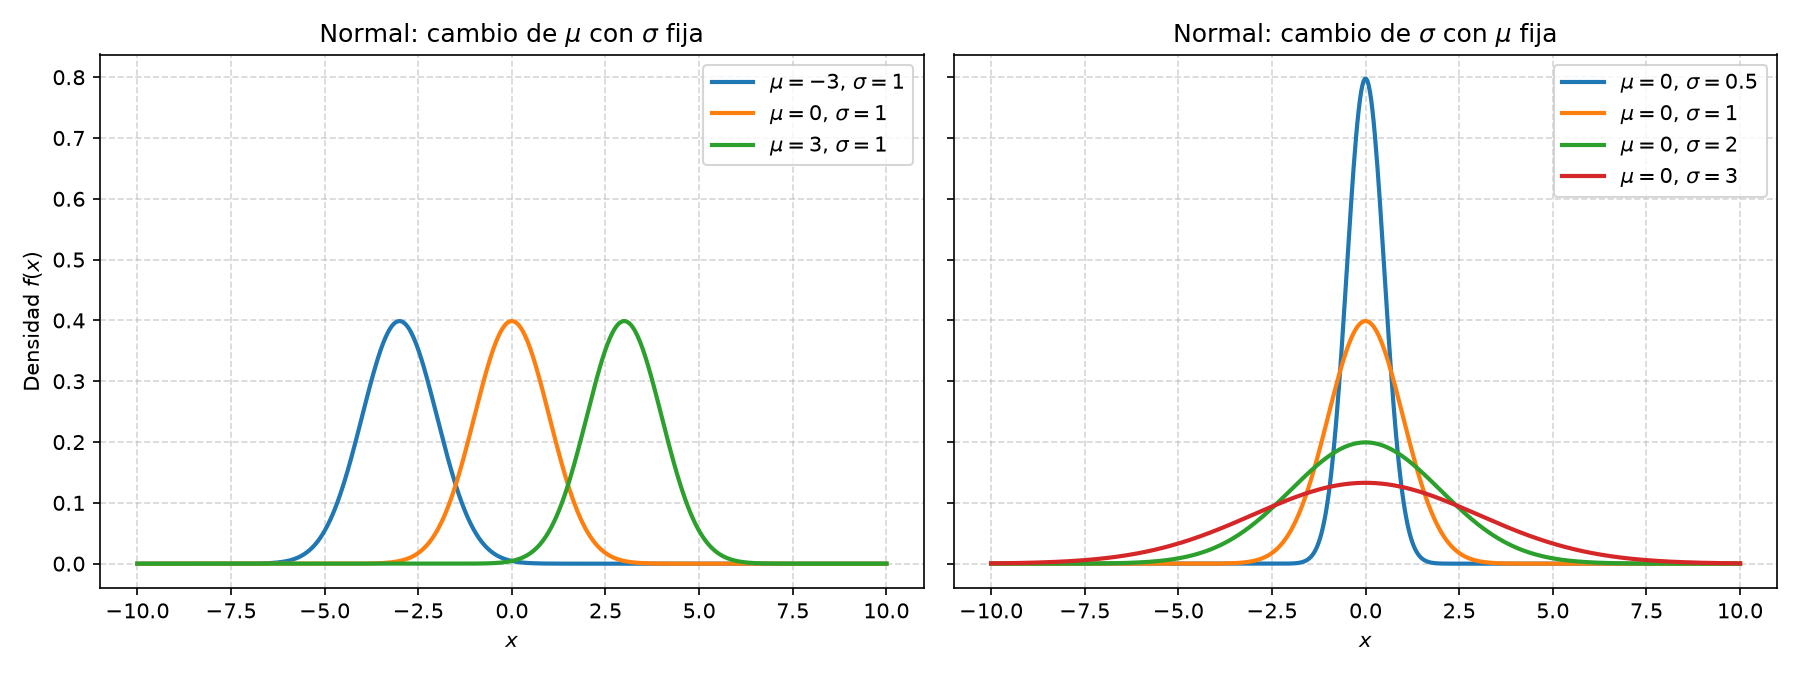
\includegraphics[width=\textwidth]{img/normal_parametros.png}
\caption{Densidad normal. Izquierda: tres valores de $\mu$ con $\sigma = 1$. Derecha: cuatro valores de $\sigma$ con $\mu = 0$.}
\label{fig:normal}
\end{figure}

Al cambiar $\mu$ (izquierda), la curva se desplaza sin deformarse: las tres campanas tienen la misma altura (0.399) y anchura. Al cambiar $\sigma$ (derecha), la curva se estrecha o se ensancha alrededor de la misma media: la altura máxima baja de 0.798 con $\sigma = 0.5$ a 0.133 con $\sigma = 3$, porque el área total debe seguir siendo 1. La probabilidad dentro de $\mu \pm \sigma$ es la misma, 0.6827, en todos los casos: $\sigma$ cambia la escala de la curva, pero no su forma.

\subsubsection{Distribución Poisson}

El Código~\ref{cod:poisson} grafica la masa de la Poisson para $\lambda = 1, 4, 10$ y 20, y compara la de $\lambda = 20$ con la normal de igual media y varianza (Figura~\ref{fig:poisson}).

\begin{codigo}[label=cod:poisson]{Tarea 3: distribución Poisson}
# lambda es a la vez la media y la varianza; al crecer, la masa se desplaza y se dispersa
# y la forma se vuelve simétrica, parecida a una normal
k = np.arange(0, 41)
lambdas = (1, 4, 10, 20)
fig, (ax1, ax2) = plt.subplots(1, 2, figsize=(12, 4.5))
ancho = 0.8 / len(lambdas)
for i, lam in enumerate(lambdas):
    ax1.bar(k - 0.4 + ancho * (i + 0.5), stats.poisson(lam).pmf(k), width=ancho,
            label=fr'$\lambda = {lam}$')
ax1.set_title(r'Poisson: cambio de $\lambda$')
ax1.set_xlabel('$k$ (número de eventos)')
ax1.set_ylabel('Masa $p(k)$')
ax1.set_xlim(-1, 35)
ax1.legend()
ax1.grid(linestyle='--', alpha=0.5)

# Aproximación normal: con lambda grande la Poisson se parece a Normal(lambda, sqrt(lambda))
lam = 20
ax2.bar(k, stats.poisson(lam).pmf(k), color='skyblue', edgecolor='black', alpha=0.8,
        label=fr'Poisson($\lambda = {lam}$)')
xc = np.linspace(0, 40, 400)
ax2.plot(xc, stats.norm(lam, np.sqrt(lam)).pdf(xc), color='tab:red', linewidth=2,
         label=fr'Normal($\mu = {lam}$, $\sigma = \sqrt{{{lam}}}$)')
ax2.set_title('Poisson con $\\lambda$ grande y su aproximación normal')
ax2.set_xlabel('$k$')
ax2.legend()
ax2.grid(linestyle='--', alpha=0.5)
guardar('poisson_parametros.png')

print("\n=== Tarea 3: Poisson, media, varianza y masa máxima ===")
for lam in lambdas:
    d = stats.poisson(lam)
    print(f"lambda = {lam:<3} media = {d.mean():.1f}  varianza = {d.var():.1f}  "
          f"masa máxima p(k) = {d.pmf(k).max():.3f}")
aprox = stats.norm(20, np.sqrt(20))
error = np.abs(stats.poisson(20).pmf(k) - (aprox.cdf(k + 0.5) - aprox.cdf(k - 0.5))).max()
print(f"Error máximo de la aproximación normal con lambda = 20 (corrección por continuidad): {error:.4f}")
\end{codigo}

\begin{consola}[label=out:poisson]{Ejecución de \texttt{act14.py}: Tarea 3, Poisson}
=== Tarea 3: Poisson, media, varianza y masa máxima ===
lambda = 1   media = 1.0  varianza = 1.0  masa máxima p(k) = 0.368
lambda = 4   media = 4.0  varianza = 4.0  masa máxima p(k) = 0.195
lambda = 10  media = 10.0  varianza = 10.0  masa máxima p(k) = 0.125
lambda = 20  media = 20.0  varianza = 20.0  masa máxima p(k) = 0.089
Error máximo de la aproximación normal con lambda = 20 (corrección por continuidad): 0.0048
\end{consola}

\begin{figure}[htbp]
\centering
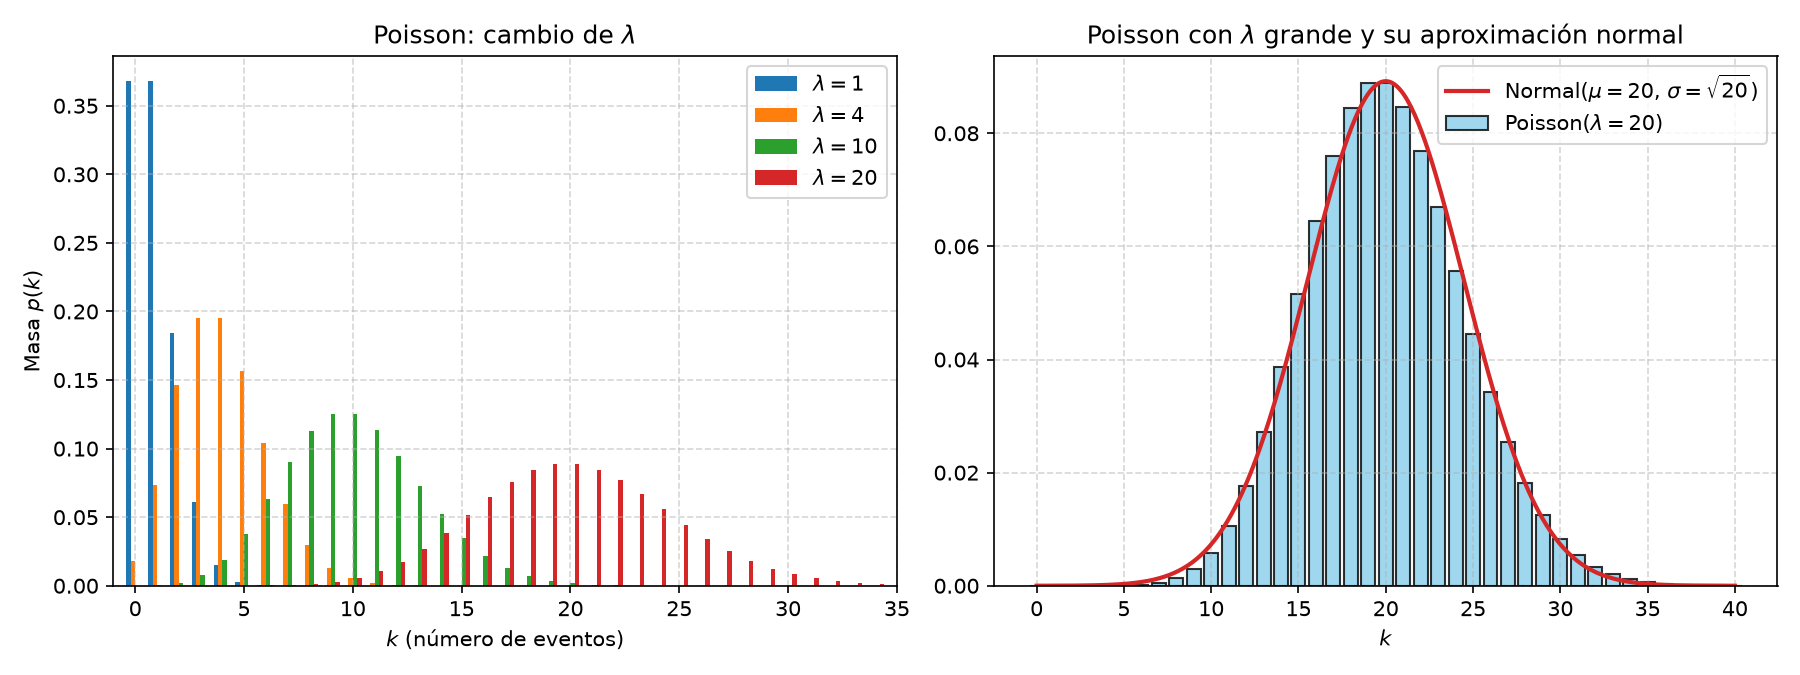
\includegraphics[width=\textwidth]{img/poisson_parametros.png}
\caption{Masa de la Poisson. Izquierda: cuatro valores de $\lambda$. Derecha: Poisson($\lambda = 20$) y la normal con la misma media y varianza.}
\label{fig:poisson}
\end{figure}

Con $\lambda = 1$ la masa se concentra en 0 y 1 (0.368 en cada uno) con una cola derecha, es decir, es asimétrica. Al crecer $\lambda$, la masa se desplaza a la derecha, la media y la varianza crecen juntas (son siempre iguales, como se ve en la salida) y la masa se reparte en más valores, por lo que su máximo baja de 0.368 a 0.089. Con $\lambda = 20$ la forma es casi simétrica y la normal con $\mu = 20$ y $\sigma = \sqrt{20}$ la aproxima bien: usando la corrección por continuidad, la diferencia máxima por valor es de 0.0048. A diferencia de la normal, en la Poisson el parámetro de forma y el de escala no son independientes: no se puede cambiar la dispersión sin cambiar la media.

\subsection{Tarea 4: Resumen}

\begin{quote}
Elegir bien la distribución es importante porque determina qué datos puede generar el modelo y qué predicciones considera posibles. En un modelo bayesiano define tanto la verosimilitud como las distribuciones previas, así que un error se propaga a la posterior y a las predicciones. La variable debe ser compatible con el soporte de la distribución: una normal asigna probabilidad a valores negativos, y una Poisson solo admite conteos con varianza igual a la media. Si no se cumple, los intervalos de credibilidad engañan y las predicciones son poco confiables. Por eso conviene escoger según el tipo de variable, verificar el supuesto con gráficos y pruebas, y sustituir la distribución cuando falle \parencite{tecnm2026_documento_fuente}.
\end{quote}

\section{Conclusiones}

Las ocho distribuciones del documento fuente se clasificaron según el tipo de variable que modelan: normal, exponencial, gamma y uniforme son continuas y se describen con una densidad, y Poisson, binomial, binomial negativa y multinomial son discretas y se describen con una masa. La tabla comparativa muestra que cada una responde a una situación distinta: tiempos de espera, conteos de eventos, éxitos en ensayos o variables simétricas.

Las gráficas muestran que los parámetros controlan la forma de manera distinta en cada distribución. En la normal, $\mu$ desplaza la curva y $\sigma$ solo cambia su escala, y la probabilidad dentro de una desviación estándar es siempre 0.6827. En la Poisson, un solo parámetro controla la media y la varianza a la vez, y con $\lambda$ grande la distribución discreta se aproxima a una normal (con un error máximo de 0.0048 en $\lambda = 20$). Esta restricción de la Poisson es la que obliga a cambiar de distribución cuando los datos tienen más dispersión que media.

En conclusión, la distribución debe elegirse por el tipo de variable y por las propiedades que se esperan de ella (soporte, forma y relación entre media y varianza), y luego verificarse contra los datos.

\referencias

\end{document}
